\documentclass[12pt, a4paper]{report}

\usepackage{fyp}

%%these packages are not really necessary if you dont need the code and proofs environments
%%so if you like you can delete from here till the next comment
%%note that there are some examples below which obviously won't work once you remove this part
\usepackage{verbatim}
\usepackage{amsfonts}
\usepackage{amsmath}
\usepackage{amssymb}
\usepackage{amsthm}
\usepackage[hidelinks]{hyperref}
\usepackage{graphicx}
\usepackage{lmodern,textcomp}

%%this environment is useful if you have code snippets
\newenvironment{code}
{\footnotesize\verbatim}{\endverbatim\normalfont}

\graphicspath{ {images/} }

%%the following environments are useful to present proofs in your thesis
\theoremstyle{definition}
\newtheorem{definition}{Definition}[section]
\theoremstyle{definition}%plain}
\newtheorem{example}{Example}[section]
\theoremstyle{definition}%remark}
\newtheorem{proposition}{Proposition}[section]
\theoremstyle{definition}%remark}
\newtheorem{lemma}{Lemma}[section]
\theoremstyle{definition}%remark}
\newtheorem{corollary}{Corollary}[section]
\theoremstyle{definition}%remark}
\newtheorem{theorem}{Theorem}[section]
%%you can delete till here if you dont need the code and proofs environments

\setlength{\headheight}{15pt}
%\overfullrule=15pt


\begin{document}


%%make sure to enter this information
\title{Pin Pointing Pain Points: Vehicular traffic flow intensity detection and prediction through mobile data usage.}
\author{Maurice Saliba}
\date{28-06-2018}
\supervisor{to insert}
\department{Faculty of ICT}
\universitycrestpath{crest}
\submitdate{28-06-2018} 

\frontmatter


\begin{acknowledgements}
your acknowledgments
\end{acknowledgements}
       
\begin{abstract}
Multi-modal originated vehicular traffic flow data can be obtained with various techniques. To what extent this data is reliable, complete, timely and readily available requires a thorough analysis of past work and currently available solutions. A novel approach consisting of an ensemble of machine learning and data-mining techniques is being proposed. 
A mobile phone usage dataset from a telecommunications provider in Malta is used first to carry out basic traffic analytics. Then an origin destination (OD) matrix based on the largest two clusters of activity per user will be computed to infer user trips between these clusters across time. Routes for these trips are retrieved with open source routing tools and obtained data pertaining to way nodes along these routes further enrich trip information. Spatial binning is then used to deduce the distribution of traffic load on the traffic network.  The OD matrix and grid network load are subsequently used to build a Neural Network predictive model. Several previous works \cite{Laurila2012,Hoteit2014} that carried out invaluable research in this field lacked on-line data in quality and quantity. They were at times compelled to devise corrective measures and carry out simulations to cater for such shortcomings. Having the luxury to avail of mobile call and data historical records will make it more possible to fine tune a better predictive model and evaluate it. To wrap up this research, industry standard visualization tools will portray AI generated traffic patterns together with flow intensity projected in the geospatial dimension. 
\end{abstract}

\tableofcontents

\listoffigures

\listoftables



\mainmatter

\chapter{Introduction}

\section{Economic development and urbanization impact on transport}

Land transport is a societal reality that is required for displacement of people for work, 
leisure and other purposes. Transport is important as well to deliver goods and services. Land transportation has undoubtedly evolved with a fast pace and late technology advancements are making vehicular transportation more efficient, less polluting, faster, safer and more comfortable. There are many land transport modes which include bus, rail and private car as the most generally used.

Economic development and urbanization comes at a cost. It surely has a direct impact on the increase of traffic congestion and all undesirable consequences it brings with it. Traffic congestion is especially synonymous with urban places where private car is the preferred mode of travelling. \cite{EUTransportDirectorate2018} mentions how traffic congestion in urban areas in the EU is costing 100 billion every year which amounts to 1\% of the EU GDP. \cite{Colak2015} ellaborates on the crippling effect on the economy because of traffic congestion. Traffic congestion amounted to 43\% (\texteuro117.9 million) of external costs in Malta in 2012, which is the origin of the mobile traces datasource used in this study \cite{Attard2015}. Other causes of external costs related to traffic include accidents, climate change, air pollution and noise which are all directly incremented by traffic congestion. No policy change scenario envisages an external cost of \texteuro151.1 million and \texteuro154.1 million for the years 2020 and 2030 respectively incurred on the economy of Malta.

In the US traffic congestion is similarly a cause of concern. Interesting but worrying facts are listed in a US mobility research done in 2015 \cite{Schrank.2015}. It states that the extra miles travelled by Americans in 2014 were 6.9 million at the cost of \textdollar160 billion. Congestion costs in the USA is on the increase. In the year 2000 it was reported to be at the level of \textdollar114 billion.

Traffic delays impact direly also the shipment industry. Travel costs increase when travel time increases.  Pick-up and delivery times are more approximative. Transport companies need to take costly measures in order to make up for this and the increase in cost is more often than not passed to the consumer  \cite{Schrank.2015} \cite{CambridgeSystematicsInc.2005}.

\section{Addressing Traffic congestion}

Car users and even public transport users (since buses cannot avoid traffic although use of it alleviates it) tend to get rather frustrated from lost time on the road. This time is deducted from a healthy lifestyle or from productivity hours. 

Driver self adaptation measures help to smartly mitigate delay times. Individual drivers can hear radio adverts or check CCTV to enquire the traffic situation before departing or even while driving for better planning. Use of software such as Google maps, Apple maps or Waze help to have an informed decision how to schedule trips and decide what route to take.  These applications might even suggest to take other transport modes because it is more convenient especially in terms of less time to get to destination.

Addressing traffic delays should be addressed within a wider scope. Efficient traffic management should be on top of government transportation agencies agenda. Traffic management is multi-faceted especially the urban one. Possible measures that can be taken by transport authorities include making different modes of transport available and encourage the public to use it. Smart technology is a good candidate to alleviate travelling frustration by giving information,instructions and control parameters that have a say on traffic. For more uptake of public transport the public for instance can be informed and educated through mobile applications.  Mobile applications can be used to make the public transport experience more efficient, practical and the preferred choice. There are other deterrents such as increases in vehicle license tax and adding of parking fees to force drivers off the road and make them use public transport or go for any generic modal shift. But these are rather unpopular measures and policy making agents are susceptible to pressure in such a way that they are less proactive to implement such measures.

Other measures to tackle traffic problems is by enforcing traffic laws. This would diminish road accidents or casual road blockages that can cause flow disruptions. CCTV road network monitoring would be helpful to inform drivers to take alternative routes. CCTV could be used also for deployment of traffic management personnel in problematic areas. License number plate recognition through camera feeds processing can be used to measure traffic flow and even to apply a toll to users in certain traffic zones as a deterrent for private car use.  Park and ride systems may shift away concentration of traffic from urban centres.  \cite{AlNuaimi2015} for instance suggests how concerted efforts can lead to smart cities by analysing static data and make infrastructural changes by opening or modifying roads. Dynamic data then would be used to manage traffic lights to alleviate congestion, inform the public through their smart phones about the traffic status and orchestrate shipping movement for the supply chain.

Investment in the transport infrastructure to expand capacity is difficult to directly justify with a simple cost benefit analysis model. Increase in road capacity might seem a simple straightforward solution to alleviate traffic.  However infrastructure alterations might not necessarily equate to easing of traffic. Such costly changes might just spatially shift the problem elsewhere or not lead to the expected result. Forecasting of the gains made by road capacity increase or any other transport system changes may be distorted if induced traffic is not taken in consideration. Induced traffic may result from changes in route choice, peak hour traffic, modal split, overall transport volume, land use and quality of public transport services \cite{Naess2012}. When formulating return on investment functions induced traffic should not be ignored.


\section{Traffic information and management systems}

Traffic management would primarily consist of a systematic approach to monitor accurately, with wide coverage what is the traffic status in the road network. In order that this information is kept relevant it needs to be constantly updated and gathered in a reliable fashion. Once such information is acquired intelligent traffic management systems architectures can be designed around static data and traffic control is based  on constant input feed stream processing. Obviously the latter is more challenging in terms of computational resources and design but is more reactive to abnormal situations such as accidents or unusual weather conditions since it is modelled on a running sample \cite{Toole2015}. Traffic related data stream processing might entail heavy real time processing of high variety data coming from multiple sources. Modern approaches such as big data based information systems become essential in order to create automated control systems that alleviate the load on the transport network.

Traffic information Systems may be based on mobile data as main source of information. These type of systems would require that mobile data collection and its processing has wide coverage, is reliable and accurate and updated with high frequency \cite{Leduc2008}. Less coverage is to be expected in rural areas where base stations are highly dispersed when compared to urban areas. Mobile vehicle geolocation cannot be used for traffic flow counts on lanes as it can be done with inductive loops. Frequency of updates refers to collection of data that probes the traffic situation (counts) and also to the amount of fresh updates users get from the traffic information systems in real time.

\section{Traveller centric traffic flow probing}

Obviously the dynamics of traffic flow is determined by the travel needs of the masses. The daily commutes of every individual impacts those of others. The interaction at large scale of all the vehicles in a time series is difficult to model and then predict how traffic is affected along the course of the day. Traffic sensors, cameras and induction loops are all sources of information that can be lead to both detect high traffic intensity or even forecast it beforehand.  However the coverage these techniques offer is limited. Camera feeds and inductive-loop detectors cannot be installed in every road of the transport infrastructure. Crowd-sourced information that gives information on mobility traces enables new approaches how to make the road infrastructure management, both inter-towns and intra-cities, smarter. Vehicles and people that are on the move become traffic measurement mediums.

Long before the information era started, spatio-temporal data on human mobility was collected in various forms and modalities. There are various reasons that raise interest in the scientific community for gathering such information. One of the methods used to gather such information is to do straightforward surveys\cite{Calabrese2013,Colak2015}. However these are expensive in terms of manual work needed to carry out and a lot of human resources are needed to gather information. Besides they could only give a snapshot of reality at a given point in time.  Generally these type of surveys are done every five to ten years \cite{Toole2015}. The data made available would be too static and increasing the frequency of survey taking would directly require more human resources assigned to the process. Given that telecommunications came into the picture and there was a wide adoption of its services at the turn of the millennium one could gather data more frequently in vaster amounts and in an automated fashion from mobile devices. The sample domain got even wider. A limitation which comes with mobile phone data is the lack of background known on the travellers. Surveys gather such information and make stratified sampling possible in order to have a more representative sample \cite{Colak2015}.

\section{Application of mobile traces analytics}

Primarily mobile traces would lead to location based services that have a wide application spectrum that go beyond solving mobility issues \cite{Hoteit2014,Calabrese2013,Gonzalez2008,Hoteit2016}. An individual's location and its relation with that of others within the context of the continuum of time is invaluable in many ways. This formidable datasource however poses a challenge. Location data, which usually comes in large amounts, has to be harvested, ingested efficiently and ideally processed in real time for the required final purpose which is value added location based services.

The range of application and branches of research abound on remote collection of mobile users' geolocation information.   To name a few applications include: traffic patterns and prediction modelling, crowd management, hotspot detection, lost device recovery, emergency rescue, use for investigative authorities,  location-based recommendation and advertising systems, contextualized information, social interaction based application, epidemiology etc.  

\cite{Calabrese2013} went even further to emphasize that such studies on human mobility patterns would be vital for better sustainable urban planning and a boost for the environment's well being given that transportation in 2004 accounted for 22\% of primary energy use.

Mobile device geolocation data surely proved to be useful to setup a platform to predict how traffic/commuting patterns evolve during different time-frames such as weekdays in contrast with weekends \cite{Steenbruggen2015}. Prediction of traffic patterns would also include jam detection \cite{Hoteit2014}.  Macroscopic monitoring and analysis of vehicle mobility through mobile traces is a wide area of study on its own which can branch in many fields of study \cite{Steenbruggen2015}. 

In this dissertation we will focus on the topic of measuring traffic flow and predict how traffic increase along time by using mobile data usage. A combination of data mining and machine learning techniques will be used to devise a data processing pipeline. This pipeline will consume raw event data records containing cell tower locations and date time and then it zooms into the main areas of activity of users, plots routes between these areas and collects spatial grid aggregate data from daily trips done along these routes from thousands of users. The dataset which is produced from this pipeline is used to train and validate a predictive model using artificial neural networks.

\section{Aims and objectives}

The problem to be tackled by this research will be traffic congestion detection and also its prediction within a specific time window. Traffic congestion can be measured through aggregate functions exercised on areas with well defined geo-fences. Traffic hotspots' data is more static unlike the location of mobile users which is less accurately traceable. The trip trajectory of an individual when compared with traffic congestion at a given point is far more non-deterministic \cite{Jarv2012}. Data aggregation of multiple users against time will produce more accurate results when predicting waiting times at a traffic hotspot then when trying to predict the trip for a given time interval and specific mobile user.

Traffic congestion analysis is tightly linked to a long list of factors. These factors are related in some way or another to mobile network determined location. It is not however excluded that the dataset is further augmented. Such factors or 'features' as most often referred to in applied artificial intelligence jargon might include but are not limited to are: number of exits at a junction point, distance from the nearest busy(a standard threshold is to be chosen on what defines 'busy' ) junction point, aggregate statistics of currently moving mobile users, historical trajectory data for drivers in the area, actual day of week, seasonality (whether it is a holiday or schools are closed), current infrastructural works which might skew the analysis, accidents records to correlate anomalies etc. Techniques that will be used as a traffic congestion metric is count of moving users per spatial bin at a given point in time\cite{Alarabi2014}. Spatial bins are geo-fenced areas in a rectangular format that enclose geospatial information. Frameworks such as Spatial Hadoop facilitate parallelized processing on large datasets in order to group data points in spatial bins for further analytics \cite{Alarabi2014}. 

We propose a systematic approach how to address the problem often stated in literature related to mobility patterns \cite{Calabrese2013,Toole2015,Hoteit2014,Alexander2015}. We are aiming to devise an accurate metric of traffic congestion and be able to forecast traffic through a model trained and tested with available mobile usage data. The real challenges resides in achieving granularity when modelling traffic given that mobile usage records' geolocation dataset is sparse and reveals the position of users with a considerable margin of error \cite{Hoteit2014,Gonzalez2008}.

\section{Dissertation outline}
This dissertation started with a section that introduces the reader to the vehicular traffic problematic nature. It continues by expanding the socio-economic impact of traffic and how it can be addressed with modern technology. At the outset it is mentioned how mobile data usage has great potential to monitor traffic conditions and to predict it across time. The following chapter "problem definition" will discuss how the problem at hand of measuring traffic and predicting from mobile usage data is not trivial. It will show where the main challenges reside in order to arrive to a viable solution. Background on traffic flow detection and prediction and an overview of related literature will be given in chapter \ref{background} "Background and literature review". The proposed method to showcase selected implementations of certain concepts inspired by literature will be elaborated in the "Methodology" chapter.  Validity and versatility of the created model will be evaluated in the "Evaluation and Results" chapter. Finally the "Conclusion and Future works" chapter will summarize what has been achieved in this work and to what extent.  In this chapter shortcomings of the proposed solution will be discussed and possible improvements and prospects for the future will be listed.



\chapter{Problem definition}

\section{Problem statement}
From this research it is required to demonstrate that it is possible to attain an accurate measure of traffic and predict traffic for different amounts of time ahead. It is required to prove that this can be possibly done by constructing a predictive model and make use of inference techniques that base themselves on data usage records collected from the mobile cellular network. As we will expand in chapter \ref{background}, the trajectory path plotted by the mobile antenna through which users are given service is far from being a true picture of the actual path of the user.  An algorithm must be devised to deduce the actual path travelled by the user for his most common trips. The predictive model must possibly predict the traffic in a reasonable amount of time since a prediction that take a long time to compute will become futile in its purpose.


\section{Research Questions}

Research will be done in a direction outlined by the questions below:
\begin{enumerate}
	\item How is it possible to extract the geolocation of main areas of activity from user's mobile data usage records?
	\item What is the best approach to analyse traffic flow over time in space? Is the resolution of mobile data usage cell tower location fit for purpose to measure vehicular traffic flow on the road network?
	\item Is it possible to model traffic flow over time with machine learning techniques that use mobile data usage or processed data derived from it? From how much time ahead can the model predict traffic flow with an acceptable margin of error in such a way that the prediction is useful and practical for trip planning and traffic management systems?
\end{enumerate}



\chapter{Background and Literature Review} \label{background}

This chapter will go over mainstream techniques and approaches that make use of mobile data for traffic flow detection and prediction.

\section{Mobile location data sources} \label{background_mobile_location_data_sources} 

Mobile location retrieval include various sources. User locations have to be recorded from cell towers mainly for billing purposes. Other records are generated when there is a location update and hand over information \cite{Calabrese2011}. Geographical coordinates of the cell tower are added with billing information. Call data records (CDR) or event data records (EDR) as they are generically referred to when they comprise other forms of activity other then calling are generated by network elements to capture and report user activity within the network. Reporting frequency and record triggering events can be configurable, allowing operators to trade off between keeping at their lowest the quantity of generated records that are hungry of storage resources and providing enough data for billing/troubleshooting purposes.
Mobile internet is the service that generates most records. As soon as the user connects to the network, a first record is generated, providing all of the available information, including which cell tower is providing the service. Since data sessions span over a long period of time, periodic updates are required, allowing billing related entities to decide whether the user may continue to make use of the service. These updates may be triggered by either of the following:
\begin{enumerate}
\item Volume - a new record is generated as the user consumes more than a pre-configured volume.
\item Time - if the user is idle, a new update record is still generated after a specific amount of time from the previous record.
\item Network Trigger - operators may decide to generate a record each time there is a specific change (for instance, a change in radio access technology)
\end{enumerate}
	
Together with call records, SMS records (messaging) and data traffic (2G/GSM, 3G/UMTS, 4G/LTE) records can also be stored. SMS records structure are similar to those of CDRs \cite{Calabrese2013}. A call data record structure would include the A-party (who is calling), the B-party (the person who is receiving the call), call duration, date and time of calls amongst other things which might not prove to be useful for location deducing purposes. The location is implicitly the sector of the base station antenna which was managing the call/sms and where ultimately the CDR has its origin. The technology of mobile data transfer (2G, 3G or 4G) the user device makes use of is negotiated depending on the strength of the signal and load of cell tower \cite{Liu2014}. The technology used will fail-over to a less faster one but stronger in signal strength if reception experienced by user weakens (example changeover from 4G to 3G and so forth). This has an implication on location detection as we will see later on. A data event record would include volume of transmitted data in the session.

Mobile device location traces have their limitations when used for vehicular traffic analyses. In contrast with surveys they lack demographics \cite{Calabrese2013,Colak2015} and market share of the mobile service provider that made the dataset available for scientific research might not be really representative of the commuting patterns \cite{Calabrese2011}. Many studies mentioned that it is important to remove bias in preprocessing of such datasets before any further processing is done \cite{Iqbal2014,Toole2015}.  Passive data gathered in the form of CDRs are not suited to extract different modes of travel, route assignment and classify detailed activity types \cite{Colak2015}.


Mobile device location data is not only limited to data that originates from cellular networks. Global positioning system (GPS) is the most reliable source of geolocation because of its higher resolution with lower margin of error. This data is generated on the device and needs to be stored and communicated from the user's mobile with his own specific authorization. Using GPS data for a mobility study is more challenging because it needs the consent of users to get such data and drains the battery really fast especially because of long signal acquisition time \cite{Wang2012}. Thus users would be reluctant to have such service running in the background on their mobiles all the time \cite{Ahas2011}. 

CDRs were the most commonly mobile location data source used in recent research \cite{Hoteit2016}. The intention of our research is to use data usage EDRs since these can have a higher temporal resolution. A CDR can be more commonly generated when a user is not moving unless he is using hands free in his car. CDRs therefore would be more suited for home and work location detection whilst data usage records would be more generated frequently both when user is moving and stationary. To our best knowledge up till today the trend is to use CDRs. There are very few research projects that rely on mobile data usage to detect vehicular traffic or predict it. Few examples in literature are  \cite{Hoteit2014,Calabrese2011}. 

Other sources of geolocation include social mobile application recorded events such as check-ins in facebook \cite{Hoteit2014}. Such data can be accessed by available APIs.

\subsection{Data format and sample structure used in literature} \label{methodoloy_sources}


It is important to analyse in depth the structure of mobile records dataset sample and the method of collection thereof in order to understand possible limitations and strengths in related research. Another topic of special interest is the use of secondary datasets used to validate results achieved modelling travel on mobile generated data. Hoteit et al utilized mobile data coming from 1 million users between July and October 2009 \cite{Hoteit2014}. The data consisted of calling and messaging parties' anonymous id together with data of when users make a data connection. Interestingly in \cite{Calabrese2013} together with data collected from the CDRs (a sample of 1 million mobile users in Massachusetts) which contain calling id, time of when call/sms is done or received and when a data session is initiated, vehicle safety inspection data is used as part of the study. This is later used to verify approximately the kilometres covered when inferred from the trajectory computed based on the user data points. Time window is 3 months long and area covered is metropolitan Boston.  \cite{Calabrese2013,Colak2015} stressed several reasons why surveys have a lot of disadvantages when compared to mobile device generated data including sample size which is smaller, update frequency and certain types of time windows that are seldom considered or not captured by surveys such as seasonality, public holidays and weekends.   

In \cite{Gonzalez2008} two datasets are used. First sample is of 100,000 individuals sub-sampled from a wider dataset population of 6 million anonymized  phone users. Again data used was id of device from which calls or sms originated or terminated and location of tower projected over time. Average area covered by cell tower was 3 km$^{2}$ with 30\% of cell towers having a coverage of 1 km$^{2}$ or less. The other dataset consisted of 206 mobile users whose location was traced every two hours for a week. The second dataset individuated irregular calling patterns noticed in the first one. Then displacements were recorded for consecutive calls in order to construct a distribution model.

\cite{Hoteit2016} use two datasets which have GPS location of 86 mobile users in various places in the world. One dataset is generated by sub-sampling the original one in order to emulate a sparse CDR dataset. Authors were forced to do this since no real CDR dataset was available for their research.  

Two different examples of tools have been found to be employed to aggregate location data. Airsage datasets were found often to be used in literature \cite{Hoteit2014, Wang2013, Calabrese2013,Leduc2008,Wang2012, Colak2015}. Basically airsage does not simply just record the tower cell sector but depending on a refined triangulation algorithm it gives a more precise location.  \cite{Hoteit2016} makes use of MACACOApp which is an app that records mobile data usage but most importantly also GPS data. As already aforementioned GPS technology gives a more accurate geolocation. However the data sample size is much more on a minor scale than that collected from raw cdrs in other studies.

\subsection{Mobile position inference from Floating cellular data} \label{mobile_inference} 

The method that makes use of mobile data connectivity with base stations is commonly referred to as floating car data or more specifically floating cellular data (FCD) for sensor data originating mainly from cellular networks. A specific technique to actually determine a user's location is based on triangulation as done by the Airsage solution \cite{Hoteit2014}. Proprietary algorithms process data received from mobile service providers and outputs refined location information to customers. It was reported that in testing carried out by Geostat Inc. Airsage got accurate classification of congested traffic 91\% of the time  \cite{Wang2012}. No technical background was made available how these algorithms get a more precise location of mobile users and this is most likely attributed to the fact that algorithms are patented.  It is stated that Airsage location computation accuracy is within 200 to 300 metres in \cite{Colak2015}. \cite{Calabrese2013} states that the degree of precision reported by AirSage is an average of 320m and median of 220m. As already aforementioned AirSage has been used in \cite{Hoteit2014} as well. In comparison \cite{Gonzalez2008} simplistically mentions that 30\% (average is \(3km^{2}\)) of the towers are placed in a density of 1 tower per square km. This roughly would mean that at most an unprocessed location retrieved from cellular location data would have a maximum error of around 500m. 

Therefore antenna/mobile tower location to which the mobile users connect with, may not be useful for all intents and purposes since it might be hundreds of metres away from the actual position. In our research we cannot make use of Airsage datasets. Such solutions must be already in accordance with local mobile network operators and currently there are no such agreements with the local providers. Therefore in this research some effort had to be dedicated to devise a simple triangulation or clustering method that can achieve more accurate mobile user location than the actual cell tower location. Since the grouping of multiple mobile users within a grid of location cells would prove to be more efficient in accurately measuring levels of traffic an essential topic to treat in traffic congestion research is spatial binning. Spatial binning basically provide geographical aggregate statistics.  MapReduce frameworks such as Spatial Hadoop exist so the expensive temporal geospatial analytics are done within an acceptable time window \cite{Wu2014,Eldawy}. Such tools would even provide the possibility of doing spatial joins that can correlate spatial features extracted from sources such as OpenStreetMaps with mobility data from a mobile usage dataset \cite{Alarabi2014}.


\section{Privacy and data anonymization} \label{data_anonymization} 


Mobile subscribers location is highly sensitive so anonymization has to come into play if legal issues are to be avoided when handling data for research purposes. For instance \cite{Laurila2012} exposes facts regarding potential privacy breach risks within datasets that have unique identifiers hashed. Methods that adds to anonymization efficiency listed in \cite{Laurila2012} are contractual binding of data users to not reverse-engineer identity together with truncation of data if in a given area enough data is available. Also \cite{Laurila2012} gives a detailed account of techniques used to hash unique identifiers. \cite{Shin} elaborates on how to use k-anonymity algorithm so that location data of a user makes his identity undistinguishable from other k-1 other users in the same region.

Another way to guarantee privacy is limiting data retention. To safeguard privacy travel paths of a specific mobile user is kept for not more than 1 day in \cite{Hoteit2014} and 2 days in \cite{Calabrese2013}. It is the norm to assign a hashed anonymous identifier to each mobile user in such method as well.


\section{Big Data, the cloud and large scale real time stream processing} \label{background_big_data}

Computing systems could not hold the pace of the vast increase in storage requirements \cite{Liu2014}. The bottleneck have been always IO reads and while cpu processing power and disk read speeds increased, data volume related to big data problems increased at a faster rate. 

Big data frameworks are suited for such scenarios. It shards the volume of data on a cluster of nodes and makes the addition of a new node in the infrastructure seamless. Failure of a node will not disrupt an ongoing computation since data will be redundant in other blocks of data replicated on other nodes in the cluster. Replacement of failing nodes is also a smooth operation in big data infrastructure. The main shift of the high performance architectural change was not how to distribute data in the network because this alone would increase network communication latency. It resides in offloading processing to the nodes where the data is located and only the resulting required information is transmitted back to a centralized node where the driver program is.

When is the data infrastructure of a system in need of a shift to the Big Data paradigm and traditional RDBMS systems cease to be effective? When you have the 3 V's which are volume, velocity and variety in the data its a recipe for big data introduction as a part of the solution. This is quite applicable to the processing of the multitude of mobility data which comes in huge amounts and need to squeeze out information in the least amount of time. Our dataset that was collected between August 2016 and September 2017 is 150G in size. Building a predictive model on this dataset of such size and retrain in real-time would require a big data solution. Currently some of the leading frameworks in this area are Hadoop and Spark. Hadoop is treated in detail in \cite{Liu2014} and revolves around the mapreduce programming model. This work shows how enormous amounts of data is stored in a distributed fashion on HDFS (hadoop file system) which is highly scalable and fault tolerant. Spark is used extensively in lambda architectures that include both nightly batch and real time batch processing. \cite{Liu2014} might not be that related to the analysis of mobility behaviour but describes well how to process mobile device generated data traffic. It also gives a good account on how to monitor the infrastructure through various metrics and tooling. There are many papers related to mobile user travel pattern prediction that make use of big data innovation  \cite{Liu2014,Laurila2012,Kurien2012}. \cite{Toole2015} states that dataset size can be an issue for computation when determining the OD matrix. In this same study parallelization is used to assign routes to trips.


\section{Origin and destination matrices computation} \label{OD_Matrices}
A consistent recurrence in traffic flow analyses literature is the study of how to deduce origin and destination (OD) locations for travelling vehicles\cite{Iqbal2014}. Many research articles confronted the problem posed by traffic congestion detection by first deducing the OD matrix \cite{Toole2015,Iqbal2014,Alexander2015,Calabrese2011,Calabrese2013,Colak2015}. In \cite{Alexander2015} OD matrices are used to generate trips and hence also give an accurate analysis of travel patterns. in \cite{Iqbal2014} the OD matrix extracted from mobile usage data is scaled up to generate an more representative OD matrix and a simulation is carried out in order to compare with traffic counts readings collected in surveys.

ODs are used to extract main activity hubs. \cite{Gonzalez2008} states that 40\% of the time users are at their two preferred locations.  Therefore most trips can be mostly explained as being  between several locations since users tend to be highly inclined to be regular in spatial and temporal terms. All this leads to safely assume that the majority of trips are between home and work. In literature it  is commonly found that locations that were likely to be recorded in OD matrices were home and work \cite{Calabrese2011,Colak2015}.  In \cite{Calabrese2011} home location is detected for user by checking which 500 metres square cell has the most activity during the night for every specific user.

\cite{Colak2015} labels zones such as home and work and tries to find purpose behind other types of trips. \cite{Colak2015} mentions how ODs are analysed in terms of stays and trips. Frequency of calls and time of day determine the labelling of these stays. It was not possible to categorize other types of stays other than home and work. So these types of stays are generally labelled as other.
\cite{Calabrese2011} puts forward the concept of virtual location which is derived from fused visited locations by the user. Calabrese devises an algorithm which localizes the centroid of important locations in a user trip that are to be labelled as the origin or destinations of particular users \cite{Calabrese2011}. The method analyses which points are in the proximity of others within a 1 km radius. 

A common occurrence in literature is to remove users that do not make enough usage. The behaviour of these is less predictable and its more difficult to generate trips from OD data. In \cite{Toole2015} users that do not make enough calls are filtered out from dataset and \cite{Colak2015} filters out users with low activity when labelling activity zones. 

Displacement errors due to sudden change of cell tower for various reasons are reported to make datasets inconsistent. \cite{Iqbal2014} reduces false displacements by using a time window of 10 minutes. The most common location in the 10 minute window was considered the actual location. A time window of 1 hour is than used to detect trips. In \cite{Calabrese2011} a low pass filter is used to minimize localization errors. To reduce sudden movements due to cell tower handover clustering is used.  \cite{Colak2015} raises the concern in a similar fashion and says that CDR data contains jumps or oscillations which is noisy. \cite{Colak2015} mentions how Airsage dataset inherently provides triangulation that gives medoids as processed data. Filtering out of noise in a Rio de Janeiro CDR dataset is done by labelling stays only if records are registered for a user for more than 10 minutes. When observing stays for users for a long period of time it is possible to get more clear patterns where the stays are actually visited by users or not. \cite{Toole2015} removes noise from mobile phone calls deduced trajectories by using the stay algorithm proposed in \cite{Zheng2011}. A 'stay' location is recorded whenever user makes a set of calls with a time window greater than a given threshold. Centroid is then calculated for set of locations that are close to each other in order to compute a better approximate location of the user. \cite{Iqbal2014} mentions that Estimation of OD matrices can be unreliable because of sampling bias. Equally \cite{Toole2015} stresses that bias needs to be removed when constructing OD matrices.

An important attribute to consider in OD matrices is its resolution since it might be important to aggregate data for statical purposes. Very few information has been found in literature on this. In \cite{Colak2015} census tracts and town boundaries are chosen for OD resolution. No justification for this choice is given tough.

Scaling methods are often used to get OD matrices that reflect reality better. In \cite{Iqbal2014} scaling factor Beta is used to get the actual OD matrix for traffic flow. The scaling factor is obtained by inputting optimization formulas, route choice probabilistic models, network data and the OD matrix in a simulation engine. The scaling is then distributed as shown in \ref{OD_scaling}

\begin{equation}\label{OD_scaling}
\textit{OD}_{ij} = \sum _{ij} (t - OD_{ij}) * \beta_{ij} 
\end{equation}

Problem is then simplified to calculate scaling factor for a set of groups based on dataset analysis rather than for every single OD.

\cite{Colak2015} uses the iterative proportional fitting (IPF) upscaling method. Here Colak determined the expansion factor for each tract and in the IPF took in consideration trips to destinations as well. In his conclusions Colak stated that the IPF Procedure to distribute user CDRs according to population might have been too simplistic of an approach.

Route selection is tightly knit as a product of OD matrices and when linked they are commonly referred to as OD trips. In \cite{Iqbal2014} route is mostly determined by a function of least travel time path. In \cite{Toole2015} Open Street Maps (OSM) which is an open source map building framework is used to infer routing. Some studies assign trips to a user when there are consecutive calls in the same day and the calls are done from different locations. Two consecutive 'stays' that are not more than 1 day apart would constitute a trip \cite{Colak2015,Toole2015}. OD matrices determined trips would not be sufficient to model traffic on a network. Microscopic traffic assignment dependent on these trip generation exercises needs to be modelled. \cite{Toole2015} for instance implements incremental traffic assignment (ITA) in which trips are added to network incrementally. Then on each iteration routes are assigned according to capacity saturation of roads. It is admitted however that Wardrop’s equilibrium  adapts better since routes are changed dynamically depending on congestion. However ITA algorithm is chosen because it is simpler to implement. \cite{Colak2015} relies on probabilistic model for traffic assignment. Departure times for trips are set according to pre-set distribution of departures.

Traffic flow metrics can be explained in terms of vehicle count per \textit{t} amount of time or even in a more descriptive way with a metric that measures travel performance as volume over road capacity V/C \cite{Toole2015}. The latter metric has more information since a road with low capacity may be more congested than another that has the same rate of traffic flow but a higher capacity. In a more elaborate metric proposed by \cite{Toole2015} a road can be possibly classified as a function of betweenness and usage. Classes are defined as connector (high betweenness and high usage), attractor (low betweenness and high usage), peripheral (high betweenness and low usage) and local (low betweenness and low usage).

Validation related to OD matrix generation is generally done by correlating the generated locations and trips to survey data. In \cite{Toole2015} survey data traffic load on road network is compared with that generated through OD matrices formed from mobile CDRs. Simulation generated routes for the latter have been produced with the ITA approach. \cite{Toole2015} states however that other methods should be further explored to removed uncertainty from the proposed techniques.

In \cite{Iqbal2014} traffic count was collected on a spread of 3 days in 13 locations and this data was used for calibration of the system.  For validation another day was used with 4 different locations. Prediction root mean square error (RMSE) and root mean square (RMS) percent errors were 335.09 and 13.59\% respectively. In \cite{Calabrese2011} evaluation was done against a tract by tract census. Euclidean distance was calculated and the distribution of the trip distance confirms Gonzalez affirmation that trips follow a random walk \cite{Gonzalez2008}. See equation \ref{label_random_walkabel}

\begin{equation}\label{label_random_walk}
P(x) = (x+14.6)-0.78^{-x/60} with R2 = 0.98  
\end{equation}

Here euclidean distance added error and to portray visually, although it might prove to be simpler, it would not give more insight on the road infrastructure use. In the OD trip analysis done by \cite{Calabrese2011} it is estimated amongst other things that a user makes 5 trips on weekdays and 4.5 during the weekend. This matches approximately the US census data which is 4.18 during weekdays and 3.86 on weekends. Study concludes that the OD matrices that are produced with the proposed methods can be of great value to those who are responsible for traffic planning.

\cite{Colak2015} carries out validation against traffic surveys and already available OD matrices from department of transportation.  However only morning sample was used for validation. \cite{Colak2015} boasts of trip generation and attraction correlation near to 1 for both cities in study namely Boston and Rio de Janeiro. The correlation with already validated datasets is highest when OD matrices are generated from aggregations done on larger polygons. \cite{Colak2015} reports OD matrix limitations. Suitability of CDRs to determine ODs is only good at a certain resolution. Best to have higher resolution for home or work location detection and aggregation within larger zones (towns or districts) for OD trips representation. OD matrices are less fitted to get information on the whole travel model which for example includes modal split information.


\section{Graph databases and Parallel graph processing}
In traffic congestion research cross-sectional snapshots of data are of little use. Historical data hoarding is imperative in order to chisel out patterns of commute and classification of traffic patterns in every region within a set of given boundaries.

Nowadays the data encountered in many IT systems' scenarios got too voluminous in such a way that normal traditional RDBMSs could not handle any more in terms of both model and performance.  NoSql entered the scene in the last ten years to cater for new challenges and together with Big data it helped to address issues such as requirement to store unstructured and semi-structured data in a schema-less form, need for high-scalability, low-latency and high performance. NoSql however has its drawbacks as well. Most of the NoSql solutions do not support ACID transactions in order to keep data consistent for example.  

Graph databases use native storage and native graph processing. They were designed to process data mining related to graph  better than relational databases. Relational Databases are most suited for problems that are well defined at the start of a project. A clear sign when to use graph database is when designing the schema it appears that a lot of joins will be needed. Graph-parallel computation gives an edge when processing is shifted on each data node of the graph. Referential integrity although useful for data integrity as the name implies comes at a dear cost. Queries and data manipulation that involves joins are slower.  Mining of highly relational entities such as mobile users location in the traffic network and the streets map make graph databases such as Neo4j an essential tool. Destination matrices should also be stored in Graph databases. Offline graph processing frameworks such as Giraph or Spark Graphx might then be useful to carry out scheduled jobs for collating information such as shortest paths and estimations of travel duration from any point A to any point B in a map grid.


\section{Model fitting to human mobility} \label{methodology_modelling}
Mathematical modelling of human mobility is important to predict with a stated certainty the location of a mobile user in time since data collected from mobile devices is sparse. Interpolation methods were used to describe human mobility patterns in \cite{Hoteit2014}. These are namely linear-interpolation, nearest-neighbour interpolation and cubic interpolation. Linear-interpolation would simply project the mobile user position at time (t) by plotting a straight line from the last previously recorded location and the one right immediately after. This method's error margin is widened if the recorded data sample are distant in what is time interval. As for the nearest-neighbour method location is placed to the previous recorded value or to the subsequent depending which is nearest on the time axis. The cubic interpolation is best explained when contrasted with the linear one. This method as perfectly stated in \cite{Hoteit2014}  is described as "shape preserving". The slopes shaping the curves are deduced from derivatives and give a less sharp demarcation and better guess depending on a series of data samples.

In \cite{Gonzalez2008} both the variation of displacements for consecutive 'steps' (call location) and the radius of gyration distribution was modelled as truncated power-law which is referred to in all the work as a levy-flight (See figure. \ref{fig:levy_flight} and equation \ref{displacement_distribution} for illustration of displacement distribution modelling). 

\begin{equation}\label{displacement_distribution}
P(\Delta r) = (\Delta r + \Delta r_{0})^{-\beta}  exp(-\Delta r/\kappa)
\end{equation} 

with exponent $-\beta$=1.75 $\pm$ 0.15 (mean $\pm$ standard deviation), $\Delta r_{0}$=1.5 km and cutoff values $\kappa|_{D_{1}}=400 km$ and $\kappa|_{D_{2}}=80 km$ 

\begin{figure}[h]	
	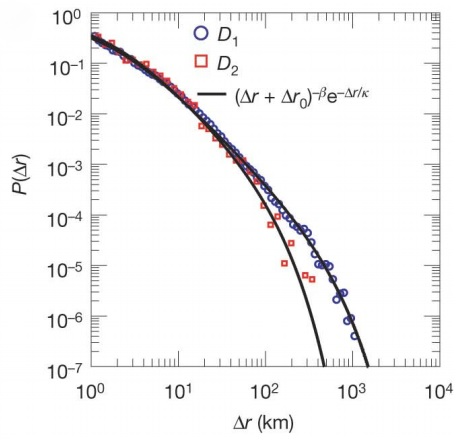
\includegraphics[scale=0.75]{truncated_power_law}
	\centering
	\caption{Truncated levy flight human motion modelling. Reproduced from \cite{Gonzalez2008}}
	\label{fig:levy_flight}
\end{figure}

This mathematical model is cited and verified in \cite{Calabrese2013}. Methodology adopted in \cite{Hoteit2016} suggested approaches how to determine home and work locations, span of movement and complete trajectory. Two datasets were compiled. The second one is a sub-sample of the first which is composed of GPS geolocation data. The sparsity of the second dataset have been mimicked by a cumulative distribution function in order to create a virtual CDR dataset. Only users with high activity were considered in order to have less irregularity. Home and work locations were determined with a mode function with catch-all time boundaries for day and night where supposedly users are either at work or home respectively. For span of movement a similar mathematical approach was adopted as the ones in \cite{Hoteit2014,Gonzalez2008}. As for the actual movement trajectory error was calculated by calculating the euclidean distance of each CDR data-point from the actual GPS recording which is nearest in time.
Some techniques were used to lessen the margin of error. Since most of the time the typical mobile phone user is static, data completion is attained by applying a list of inference rules for which different results are achieved when estimating users location, hence the name of the paper "filling the gaps".

An issue have been raised in \cite{Calabrese2013} about detecting a lot of trips in very short distance which do not tally with statistical data given by surveys. This is explained as being caused by fluctuating random connections with towers which spatially misplace the user when in reality he is not actually physically moving. This issue was tackled by mathematically creating so called by \cite{Calabrese2013} 'virtual locations' (a mass/group of traced positions in a given radius of Airsage resolution) and actually recording a movement when user moves from a virtual location to the other. Calabrese limits static location detection to the home location and the process how to manage to get each user's location is similar to that expounded in \cite{Hoteit2016}. In a novel style this work studies the relationship between total trip length calculated from mobile phone location data and vehicle kilometres travelled (VKT) and urban features such as entropic type, population density, intersection density, average distance to non-work destinations, distance to subway stations and highway exits. These urban features were derived from US Census of 2000 and activity travel surveys.

Estimation of load error is proportional to concentration if users in a given block \cite{Hoteit2014}. When error is less than 1 km a probability of 80.78\% of being within commonly travelled territory contrasts with a probability of 19.22\% when user goes outside of it. From the opposite perspective the probability of being inside radius of gyration given error is high is 40.25\% and that of being outside is 59.75\%.

\cite{Calabrese2013} boasts of 49.40\% of mobility variation can be explained for individual mobile users and 56.48\% for vehicle associated mobility in terms of trip length.    

In \cite{Gonzalez2008} results point to the phenomenon that the greater is the radius of gyration the less symmetric in shape is the probability density function which gives the probability of a user being in a given location (x,y). Also the margin of error increases similarly as stated in \cite{Hoteit2014}. It is also shown how individual mobility is well described by a levy-flight. Also a probability density function has been implemented to give the likelihood a user is at a certain given place in time.

The techniques used to further refine the location based on the assumed location home interval gives results in the range of 92\%-95\% of cases within 100m \cite{Hoteit2016}. Techniques will produce large errors (in the range of 50km) when user travels long distances and may not return to home location during the usual time interval.

Error distance from trajectory depends on radius of gyration \cite{Hoteit2014}. Interpolation methods are found to be most suited depending on distance from centre of mass. Nearest neighbour is most suited for $r_{g}$ less than 3 km. Between 3 km and 10 km both linear and cubic interpolations perform well. For commuting travelling patterns trajectory is best estimated with a cubic interpolation.
Interesting insights are contributed in \cite{Calabrese2013} where it is stated that job accessibility and distance to non-work destinations are inversely proportional to total trip length. Distance from subway does increase trip length for individual mobile users but it does not impact vehicle use. This means that subway commodity does not necessarily decrease vehicle use in the surrounding radius. Vehicular trip length decreases when correlated with increase in intersection density but not so for individual mobile users. Urban entropy and population does significantly impact trip length. Thus this study can help a lot in urban planning and large scale policy making.
\cite{Hoteit2016} affirms that the solution of data completion augmented by the placing of users in their home location at inferred intervals of time produces better results then what was achieved in literature.

There are many approaches in literature how to classify group mobility patterns under specific categories.
\cite{Hoteit2014} segments mobile users depending on how much stretched is the radius of gyration (\(r_{g}\)). The different distinguished categories of users are listed as sedentary, urban, peri-urban users and commuters. Classification boundary was decided upon steep changes in the cumulative distributed function of the radius of gyration. Respectively they fall in the ranges \(r_{g} <= 3km, 3km < r_{g} <= 10km, 10km < r_{g} <= 32km, 32km < r_{g}\). This radius of gyration (see eq. \ref{radius_gyration}) is the notion outlined by the sum of all displacements from the centre of mass divided by the number of trips. This parameter describes how distributed are the trips far away from the zone where the user mostly frequently returns. Repeated utilization of this mathematical notion is found in \cite{Hoteit2014,Gonzalez2008,Hoteit2016}.

\begin{equation} \label{radius_gyration}
r_{g} = \sqrt{\sum _{i=1}^{n}({\stackrel{\to }{p}}_{i}-{\stackrel{\to }{p}}_{centroid})^2}
\end{equation}

where 

\begin{equation}
{\stackrel{\to }{p}}_{centroid} = \sum _{i=1}^{n}{\stackrel{\to }{p}}_{i}
\end{equation}

In \cite{Hoteit2016} the hypothesis that an individual tends to be found with high probability at his home or place of work makes the authors to come out with so-called 'stop-by' categories. The stop-by categories are stop-by home which is demarcated by the night time interval where a user is expected to be at home. stob-by-flexhome is a refinement over and above stop-by-home were night time interval varies per user. Stop-by-spothome fills data lacunas or corrects errors when there are exceptional errors where user is expected to be in home location as indicated by previous category.


\section{Prediction methods}

{works in progress}

Prediction of traffic results have to take in consideration where the model is being used for forecasting. \cite{Sommer2013} states for example that it is easier to predict traffic in highways rather than in urban areas since traffic tends to be smoother.





\chapter{Methodology}

As outlined in the problem statement this research has to extract meaningful features from mobile data usage that would serve as the basis to build a traffic flow model. Before getting direction on what algorithm to use in order to map raw data and translate it into traffic flow metrics a thorough exercise of familiarization with the data was due. A feasibility check had to be carried out on whether it was possible that by devising an algorithm a direct relationship is established between data and traffic flow. If data would have proven to be too sparse both temporally and spatially a decision would needed to have been taken to either augment the dataset with other features such video streams with ANPR, call data records, past datasets, incident reports and anything related to road transport which would convey information on human mobility patterns. In this chapter we will elaborate how we investigated the possible approaches and how we decided to dig deeper with some chosen techniques rather than others depending on level of confidence.

\section{Mobile data collection and structure}

The dataset was made available from GO Plc Malta. The dataset recorded ranges from October 2016 to September 2017 which is a full year of data. Number of distinct cells amount to several thousands but distinct cell locations amount to only a few hundreds since a cell tower shares antennas for different technologies (Exact numbers cannot be disclosed due to commercial reasons).

As stated by the provider of the dataset, EDR/CDR records are generally buffered to file on the network element. Files are closed periodically, generally every 1 to 5 minutes. Files are then collected and processed by the mediation platform, which parses, enhances, and extracts all of the necessary information from these records. New files are then sent towards billing and other entities as per required. It normally takes around 10 minutes for an EDR/CDR to be within the data-warehouse, hence available for further processing. However mobile operator stated that polling frequency can be increased as needed.

Unique data usage users amount approximately to 108 thousand for the month of October 2016. This month was chosen because it has heavy traffic because schools start in their full sway and university students start to travel with their cars adding to the load of traffic. This sample would be roughly representing half of the provider's subscriber base which is just over 100 thousand. This figure was derived from all the distinct users that make call or use data. Therefore the number of data users that are in the sample is roughly half of the whole set of users. One must take note however that all these data users in this study might not necessarily contribute in a directly proportional manner to the number of vehicles on the move at a certain point in time. There might be static users, users who are just passengers in the car, users that have more than one device and user that make use of other means of transport. All these facts must be taken in consideration when setting up the proposed solution and evaluating results.

%TODO - Here to correlate with MCA data on data usage and subscriber base.

\begin{table}[h]
	\centering
	\resizebox{\textwidth}{!}{

\begin{tabular}{|l|p{5cm}|c|}
	\hline 
	\textbf{Data item} & \textbf{Description} & \textbf{Example value} \\ 
	\hline 
	 A\_NUM & user hashed identifier. & 5a8bd7889fb3051b10f249a5554c803a \\ 
	\hline 
	TIMESTAMP & date and time of usage. & 2017-01-01 00:00:00.000 \\ 
	\hline 
	SOURCE & Type of Record. Data or Voice. & DATA \\ 
	\hline 
	CELL\_ID & Cell identifier & 3073 \\ 
	\hline 
	TOWN & Cell town & Paola \\ 
	\hline 
	DURATION & Duration of call or data session in seconds & 60 \\ 
	\hline 
	VOLUME & Volume of data used in session in kilobytes. 
	Applicable only for records of data usage. & 324.34 \\ 
	\hline 
	LONGITUDE & longitutidnal coordinate & 14.50664 \\ 
	\hline 
	LATITUDE & latitude coordinate & 35.87 \\ 
	\hline 
	RAT\_TYPE & Network technology & LTE \\ 
	\hline 
\end{tabular} }
\caption{Data Dictionary of mobile usage raw dataset} 
\end{table}


\section{Dataset preliminary analysis}

Total number of records of any given type for the month of october 2016 was 125 million. 78\% of these records are data usage records. This at face value gives an indication that there is a four fold higher frequency of location records of data usage type then with calling data records. This evidently gives an edge on other research that used calling data records as their data source since the polling of users location is less sparse.

%TODO - number of sessions per hour for data users
%TODO - usage of data during the day and durng the night
%TODO - distribution of data usage (variance) per hour
%TODO - distribution o f


\section{Algorithm Selection}

One of he most challenging tasks involved in this study was to assign vehicular traffic to the road network depending on surrounding cell tower traffic in a time series.

The first approach that we tried to investigate is to relate the cell tower data by snapping it to the road infrastructure mesh depending from which direction the vehicle is coming. Various APIs are available to retrieve nearest road from an input geographical location. We had no prior knowledge on how cell tower transmission is configured. There are many settings which might determine the range of the cell tower including frequency, rated power, height of tower etc. Therefore the range of the cell towers was not known. A method to roughly estimate range was to calculate the average distance from the nearest \textit{k} neighbouring towers for all cell towers. However from samples taken from the dataset available of the cell towers across Malta the variance seemed quite high ranging from an inter-distance of 150m in urbanized areas to several kilometres in rural areas (Cell tower locations map for all the country not being shown since it is sensitive commercial data). Further to this from the analytical perspective it was decided to plot the cell towers' on the map and check if their distribution pattern would make it feasible to snap a data record cell tower location to the nearest road or area polygon. Thus here it was taken as an assumption that the area around cell towers will be be given service with equal range from each tower. Allowance for overlapping was also taken in consideration. It is evident from figure \ref{fig:cell_towers_distribution} that a lot of roads would be included in the range of a cell tower so it would have been difficult to devise an algorithm to derive trajectories and traffic flow counts from cell tower location data. Given that there are a lot of unknowns including how handover procedure is handled in specific areas and the actual range of cell towers the solution path of snapping to nearest roads depending on EDR coordinates was discarded. Such an approach would might have made it too impractical to assign traffic to traffic junctions, roads or polygon areas and the probability of inaccurate results was high.

\begin{figure}[h]	
	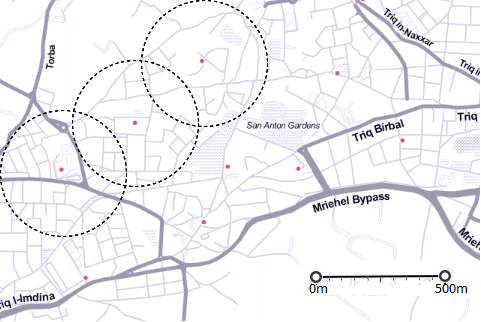
\includegraphics[scale=0.75]{cell_towers_distribution}
	\centering
	\caption{Cell tower range distribution. Red dots are cell tower locations and dotted line is the estimated range.}
	\label{fig:cell_towers_distribution}
\end{figure}

Another approach would have been to simulate traffic by inputting statistical information on travel patterns retrieved parameters from the dataset. Another input to the simulation based traffic model would have been an OD matrix that will be discussed in section \ref{clustering}. Toledo et al. \cite{Toledo2004} mentions that OD flows are an important input to simulation models but an accurate OD matrix is difficult to acquire. An example of such implementation can be found in \cite{Hirai2015}. In this study electronic toll collection data is used to form an initial OD-Matrix. This OD matrix is further optimized by optimizing a model that gets observed detector data and a simulation based on current OD, computes the least cost difference and optimizes the OD matrix depending on result. This process is iterated until an acceptable coefficient of determination is achieved. Simulation models generally give two types of outputs namely a visual simulation of traffic flow on a map and textual statistical output that can include metrics such as traffic delays, gap distances, speed and overall trip distance travelled by vehicles.

While macroscopic traffic simulators seem promising for motorways environments they are found to be less suitable for urban scenarios \cite{Bazghandi2012}. Urban environments have a lot of conflicting traffic flows caused by the numerous junctions and small roads that feed and attract traffic from the road network. Also such simulators require accurate OD matrices which cannot be achievable from our dataset. In our research we also tried to focus on the macroscopic level since we had a dataset that have ample coverage at our disposition especially in urban areas.    

%TODO - read and add notes from Macroscopic Traffic Flow Model Calibration Using Different Optimization Algorithms



\section{Main activity hubs extraction and displacement error removal through clustering}\label{clustering}

Clustering is a machine learning unsupervised technique used to classify entities which have similar features. The clustering is done depending on the algorithm and hyper-parameters that control the grouping process. Two clustering techniques that were checked for their appropriateness to this research were k-means and DBSCAN. k-means algorithm is highly popular especially for first analysis of datasets because it is simple to implement and highly efficient. The main drawback of k-means clustering is the fact that you need to select the number of clusters you need to find a priori. Then a number of centroids equal to the number of targeted clusters are randomly chosen. The algorithm starts to find the nearest neighbours based on a distance metric until finally the clusters are formed. This process is done iteratively until the ideal set of centroids with the least root mean square error are found. Also something important to note is that clusters tend to be spherical in nature. This would be highly visible of 2D clusters are plotted on a graph.

DBSCAN (density based spatial clustering of applications) has an edge on k-means and is mostly suited to our research since it does not need to set the number of clusters that we are after for each user, it finds clusters of non-spherical nature and leaves noisy elements out of the computed clusters. DBSCAN has three main hyper parameters to set namely minimum points, radius and distance metric. The algorithm is more sensitive to density rather than to aggregate distance of surrounding points. Basically the algorithm finds core points that have the required minimum points in its neighbourhood dictated by the distance metric. The points that are in this cluster but are not core points are referred to as boundary points. If core points' clusters overlap each other they form one single cluster hence the non-spehrical shape of the cluster.


This makes it a preferred candidate for clustering since our aim is to find dense clusters of activity and random locations visited by users are of no interest and need to be filtered out. 

%TODO- DBScan - check C:\Users\maurice.saliba\Google Drive\MASTERS\COURSES\SEMESTER ONE\MACHINE LEARNING\EBOOKS\SebastianRatschka

%TODO - compare dbscan to k means -> ChakrabortyNKNagwaniLopamudraDey2011

%TODO - what is the Distribution of the first two clusters on the whole data set.

%TODO - Top two activity locations extraction. What about the third one? Get distribution per user and possible filtering on distribution. Assuming that the top two activity locations for each user are the home and work location.

Given the nature of the data it was important 

%TODO - read Dynamic clustering and propagation of congestion in heterogeneously congested urban traffic networks



\section{OD Matrix Trip Generation}

Routing retrieval vs snapping to grid

duration of steps
heuristics

Individual commuting patterns.
irregular commuting patterns filtered out from analyzed dataset.

\section{Traffic flow aggregation through spatial binning}


\section{Dimensionality Reduction}

\section{Traffic flow modelling and prediction}














\chapter{Evaluation and Results}
\section{Section Name}
Mobile users averaged location calculation, estimated path trajectory and predicted traffic congestion points are basically the targets aimed for in this research project which have to be evaluated. The pivotal point here is to have a ground truth to be able to evaluate properly the obtained results. As already aforementioned in section \ref{methodology} this ground truth can be gathered from tailor made applications that collect GPS data from voluntary users. Other data sources to contrast with are actual travel diaries taken by users and traffic counts compiled from video camera captures.
All the three areas required to be evaluated need to have a uniform way how to positively assess as a good prediction or bad prediction. A way how to do is is to break down the used geographical map in a grid of arbitrarily placed cells with a specific stipulated resolution which should not be neither too big and nor too small. A root mean square cost or a cross-entropy cost function may be used in order to calculate how off-mark is the prediction when testing. A confusion matrix would be useful to visualize in a tabular fashion were the models are getting it wrong in terms of particular grid cells. Metrics used for evaluation could include an F-Measure which is a summary statistic of precision and recall and is parametrized in such a way to give different importance to precision and recall as required.

\chapter{Future Work}
\section{Section Name}
%TODO - to statisitically model route trip choice for OD matrix coordinates by eventually checking registration of users along the route taken and estimating likely route taken.

\chapter{Conclusion}
 The approach taken is systematic so that the research passes through gradual stages in such a way that we build on top of previous analyses and prototypes. Targets of this research include extraction of behavioural patterns of traffic encountered on the level of the isolated individual, subset of individuals, locality, specific time events and specific traffic hotspots. As described at the outset the main aim is not to trace the mobility of users but rather to predict estimated traffic congestion points and computation of duration for a travelling path given a starting point and a destination. Ideally if the users are highly predictable and stick to a regular travelling pattern they might be automatically notified when they are actually going to travel, how much its going to take them in terms of duration and suggestions are given to take different alternative routes which are less costly in terms of business. 

\appendix

\chapter{This chapter is in the appendix}
\section{These are some details}
%%example of the code environment
\begin{code}
this is some code;
Make sure to use this template.
\end{code}


\bibliomatter
\bibliographystyle{abbrv}
 \bibliography{references}
 
\end{document}
